\documentclass[11pt]{article}
\usepackage[margin=1in]{geometry}
\usepackage{amsmath,amssymb,amsthm}
\usepackage{graphicx}
\usepackage{hyperref}

\newtheorem{theorem}{Theorem}
\newcommand{\R}{\mathbb{R}}
\DeclareMathOperator*{\argmin}{arg\,min}

\title{A Sample Paper for the Editor}
\author{Author One \and Author Two}
\date{\today}

\begin{document}
\maketitle

\begin{abstract}
This is a small sample project used to try the editor. It has a main file,
an included section, a bibliography, a figure, and some math.
\end{abstract}

\section{Introduction}
\label{sec:intro}
Typesetting matters. This section lives in its own file to test \verb|\input| and
problem locations in included files. See Section~\ref{sec:method} for the method.

\section{Method}
\label{sec:method}
We minimize the loss
\begin{equation}
  \mathcal{L}(\theta) = \sum_{i=1}^{N} \lVert y_i - f_\theta(x_i) \rVert^2 + \lambda \lVert \theta \rVert_1 ,
  \label{eq:loss}
\end{equation}
where $\lambda > 0$ controls sparsity and $\theta \in \R^d$. Equation~\eqref{eq:loss} is \emph{convex} when
$f_\theta$ is linear.\footnote{Nonlinear models are left to future work.}

\begin{itemize}
  \item First, initialize $\theta_0 = 0$.
  \item Then iterate until \textbf{convergence}:
  \begin{enumerate}
    \item compute the gradient;
    \item take a step of size $\eta$.
  \end{enumerate}
\end{itemize}

The update rules are
\begin{align}
  g_t &= \nabla \mathcal{L}(\theta_t), \\
  \theta_{t+1} &= \argmin_{\theta} \; \langle g_t, \theta \rangle + \tfrac{1}{2\eta} \lVert \theta - \theta_t \rVert^2 .
\end{align}

\begin{theorem}[Convergence]
If $\mathcal{L}$ is $L$-smooth and $\eta \le 1/L$, the iterates converge at rate $O(1/t)$.
\end{theorem}

\section{Results}
As discussed in Section~\ref{sec:intro}, our approach builds on \highlight[comment={Cite the original method here too?}]{prior work}~\cite{knuth1984}.
Figure~\ref{fig:plot} \replaced{shows}{depicts} the two curves. Code is at \url{https://example.org/code}; see also
\href{https://example.org}{the project page}. We improved accuracy by 12\% \ldots

\begin{figure}[t]
  \centering
  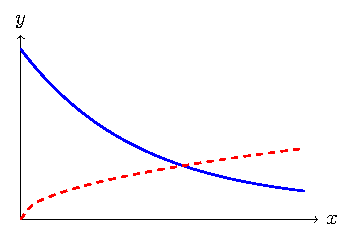
\includegraphics[width=0.6\linewidth]{figs/plot}
  \caption{Loss (blue) and accuracy (red) over training.}
  \label{fig:plot}
\end{figure}

\bibliographystyle{plain}
\bibliography{refs}
\end{document}
